\section{Тема 12}

\subsection{Подграфи. Индуцирани подграфи}

\begin{definition}
    Нека \(G = (V, E)\) е граф. \textbf{Подграф} на \(G\) е всеки граф \(G' = (V', E')\), такъв че 
    \(V' \subseteq V\) и \(E' \subseteq E\).
\end{definition}

\begin{note}
    За да бъде \(G'\) подграф на \(G\), не е достатъчно да бъде изпълнено \(V' \subseteq V\) и \(E' \subseteq E\).
    Всяко ребро в \(E'\) трябва да има за краища върхове, които са във \(V'\). Това прави \(G'\) граф.
\end{note}

\begin{example} % TODO: example
    За графа \(G_1\) имаме негов подграф \(H' = ({u, v, w, y, z}, {e_1, e_5})\):
    \begin{center}
        \begin{tikzpicture}[node distance={15mm}, thick, main/.style = {draw, circle}] 
            \node[main] (1) {$u$};
            \node[main] (2) [above right of=3] {$v$};
            \node[main] (3) [below right of=1] {$w$};
            \node[main] (4) [below left of=3] {$x$}; 
            \node[main] (5) [below right of=3] {$y$};
            \node[main] (6) [above right of=5] {$z$};
            \draw (1) -- node[above] {\(e_1\)} (2);
            \draw (1) -- (3);
            \draw (1) -- (4);
            \draw (2) -- (3);
            \draw (2) -- (5);
            \draw (3) -- (4);
            \draw (3) -- (5);
            \draw (4) -- (5);
        \end{tikzpicture} 
    \end{center}
    Нека \(H'' = ({u, v, w, y, z}, {e_6})\). Тогава \(H''\) не е подграф на \(G_1\) понеже единият край 
    на реброто \(e_6\), а именно връх \(x\), не е в множеството \({u, v, w, y, z}\). С други думи, \(H''\) 
    изобщо не е граф.
\end{example}

\begin{definition}
    Нека \(G = (V, E)\) е граф и \(U \subseteq V\). Подграфът на \(G\), \textbf{индуциран от U}, 
    е  графът \(G' = (U, E')\), където \(E' = \{(u, v) \in E | u \in U \land v \in U\}\).
\end{definition}

\begin{note}
    Индуцираният подграф е графът, чието множество върхове е \(U\) и чието множество ребра са точно тези 
    ребра на \(G\), на които и двата края са в \(U\).
\end{note}

\begin{definition}
    Нека \(G = (V, E)\) е граф и \(E' \subseteq E\). Подграфът на \(G\), \textbf{индуциран от E'}, е 
    графът \(G' = (U, E')\), където \(U = \{u \in V | \exists e \in E' \exists x \in V: e = (u, x)\}\).
\end{definition}

\begin{example}
    Нека имаме подм-вото от върхове \({u, w, y}\). Тогава подграфът, индуциран от \(\{u, w, y\}\), е 
    \((\{u, w, y\}, \{e_3, e_8\})\).

    \begin{center} % TODO: graph
        \begin{tikzpicture}[node distance={15mm}, thick, main/.style = {draw, circle}] 
            \node[main] (1) {$u$};
            \node[main] (2) [above right of=3] {$v$};
            \node[main] (3) [below right of=1] {$w$};
            \node[main] (4) [below left of=3] {$x$}; 
            \node[main] (5) [below right of=3] {$y$};
            \node[main] (6) [above right of=5] {$z$};
            \draw (1) -- node[above] {\(e_1\)} (2);
            \draw (1) -- (3);
            \draw (1) -- (4);
            \draw (2) -- (3);
            \draw (2) -- (5);
            \draw (3) -- (4);
            \draw (3) -- (5);
            \draw (4) -- (5);
        \end{tikzpicture} 
    \end{center}
\end{example}

\subsection{Свързаност и свързани компоненти в неориентирани графи}

\begin{definition}
    Нека \(G = (V, E)\) е граф. За всеки два върха \(u, v \in V\) казваме, че \(u\) и \(v\) са 
    \textbf{свързани}, ако съществува \(u-v\) път.

    \(G\) е свързан, ако всеки два върха в него са свързани.
\end{definition}

\begin{note}
    Нека \(Q_G \subseteq V \times V\) е следната релация:
    \begin{align*}
        \forall u, v \in V: uQ_Gv \iff u \text{ и } v \text{ са свързани}.
    \end{align*}
    Тази релация е \textbf{релация на достижимост} в/у \(G\).
\end{note}

\begin{lemma}
    Релацията на достижимост е транзитивна.
\end{lemma}

\begin{proof}
    Ще покажем, че за всеки 3 върха \(u, v, w\) е изпълнено, че ако има \(u-v\) път \(p\) и \(v-w\) път \(q\), 
    то има \(u-w\) път \(r\).

    Б.О.О., нека \(p\) е най-къс \(u-v\) път и \(q\) е най-къс път \(v-w\) път. Нека връх \(b\) е 
    най-близкият до връх \(u\) в \(p\) от \(V(p) \cap V(q)\). Тогава \(b\) е най-близкият до връх \(w\) в 
    \(q\) от \(V(p) \cap V(q)\). Нека \(p'\) е подпътят на \(q\) между \(b\)и \(w\) включително. Тогава 
    \(r = p' \cup q'\) е прост път между \(u\) и \(w\), тъй като \(V(p') \cap V(q') = \{b\}\).
\end{proof}

\begin{note}
    Нека \(R_G \subseteq V \times V\) е следната релация:
    \begin{align*}
        \forall u \in V: uR_Gv \iff u \text{ и } v \text{ са съседи}
    \end{align*}
    Тази релация се нарича \textbf{релация на съседство} в/у граф \(G\), която е антирефлексивна, 
    симетрична и не е транзитивна.
\end{note}

\begin{lemma}
    Релацията \(Q_G\) е рефлексивно и транзитивно затваряне на \(R_G\).
\end{lemma}

\begin{note}
    Щом \(R_G\) е симетрична и \(Q_G\) е рефлексивно и транзитивно затваряне на \(R_G\), то \(Q_G\) е 
    рефлексивна, симетрична и транзитивна. Тогава \(Q_G\) е релация на еквивалентност. Нейните класове на 
    еквивалентност са множества от върхове, във всяко от които всеки два върха са свързани, но никои 
    два върха от различни класове не са свързани.
\end{note}

\begin{definition}
    Нека \(G = (V, E)\) е граф и \(Q_G\) е релация на достижимост в/у \(G\). Подграфите на \(G\), 
    индуцирани от класовете на еквивалентност на \(Q_G\), се наричат \textbf{свързани компоненти} на \(G\).

    \underline{Алтернативно определение:} свързаните компоненти на граф са максималните по включване 
    свързани графи.
\end{definition}

\begin{example} % TODO: example
    
\end{example}

\subsection{Силна и слаба свързаност, силно свързани компоненти в ориентирани графи}

\begin{definition}
    Нека \(G = (V, E)\) е граф. За всеки два върха \(u, v \in V\) казваме, че \(u\) и \(v\) са 
    \textbf{свързани}, ако съществува път от \(u\) до \(v\) и съществува път от \(v\) до \(u\).

    \(G\) е \textbf{силно свързан}, ако всеки два върха в него са силно свързани.
\end{definition}

\begin{example} % TODO: example
    
\end{example}

\begin{note}
    \textbf{Релацията на силна свързаност} е релация на еквивалентност, защото е:
    \begin{itemize}
        \item рефлексивна, защото всеки връх е силно свързан със себе си чрез тривиален път с дължина 0
        \item симетрична
        \item транзитивна, защото ако \(u\) и \(v\) са силно свързани и \(v\) и \(w\) са силно свързани, 
        то \(u\) и \(w\) също са силно свързани
    \end{itemize}  
\end{note}

\begin{definition}
    Нека \(G = (V, E)\) е ориентиран граф. Подграфите на \(G\), индуцирани от класовете на еквивалентност 
    на релацията на силна свързаност, се наричат \textbf{силно свързани компоненти} на \(G\).

    \underline{Алтернативно определение:} \textbf{силно свързаните компоненти} са максималните по включване 
    силно свързани подграфи.
\end{definition}

\begin{example} % TODO: example
    
\end{example}

\begin{definition}
    Нека \(G = (V, E)\) е ориентиран граф. Нека \(H\) е съответния му неориентиран граф. 
    Подграфите на \(G\), индуцирани от класовете на еквивалентност 
    на релацията на силна свързаност в/у \(H\), се наричат \textbf{слабо свързани компоненти} на \(G\).

    \underline{Алтернативно определение:} \textbf{слабо свързаните компоненти} са максималните по включване 
    подграфи на \(G\), м/у върховете на които няма пътища в никоя посока.
\end{definition}

\begin{example} % TODO: example
    
\end{example}

\subsection{Оцветяване на графи}
Нека \(G = (V, E)\) е граф.

\begin{definition}
    Оцветяване на върховете на G (или просто оцветяване на G) е функция \mexpr{f: V \to C}, където 
    C е множество от цветове и е изпълнено, че \mexpr{\forall (u, v) \in E: f(u) \not = f(v)}.
\end{definition}

\begin{note}
    Има смисъл оцветяването да е сюрекция, за да няма неизползвани цветове.
\end{note}

\begin{definition}
    Минималният брой цветове, с които можем да оцветим даден граф G, се нарича \textbf{хроматично число} 
    на G (бележим го с \(\chi(G)\)).
\end{definition}

\begin{definition}
    Оцветяване на ребрата на G е ф-я \mexpr{h: E \to C}, където C е множество от цветове и е изпълнено, че 
    \mexpr{\forall e \in E \forall e' \in J(e): h(e) \not = h(e')}.
\end{definition}

\begin{definition}
    Минималният брой цветове, с които можем да оцветим ребрата на даден граф G, се нарича 
    \textbf{хроматичен индекс} на G и се бележи с \(\chi^{'}(G)\).
\end{definition}

\subsection{Планарност на графи}

\begin{definition}
    Планарно вписване на мултиграф е всяка наредена двойка (U, E), където \mexpr{U = \{u_1, ..., u_n\}} е 
    непразно множество от точки в равнината, наречени планарни върхове, а \mexpr{E = \{s_1, ..., s_m\}} е 
    множество от отворени или затворени криви в равнината, наречени планарни ребра, като трябва да бъдат 
    изпълнени следните условия:
    \begin{itemize}
        \item за всяко планарно ребра, ако е отворена крива, то двата му края съвпадат с точно два от 
        планарните върхове, а ако е затворена крива, то точно една точка от него съвпада с някой планарен връх
        \item планарните ребра не се пресичат с изключение на това, че може да имат общи планарни върхове
    \end{itemize}
\end{definition}

\begin{definition}
    Нека \(G = (V, E)\) е мултиграф. G е планарен \totw съществува планарно вписване на мултиграф (U, S) такова, че:
    \begin{itemize}
        \item съществува биекция \mexpr{\Phi: V \to U}
        \item съществува биекция \mexpr{\Psi: E \to S}, такава че \mexpr{\forall e \in E}:
        \begin{itemize}
            \item ако реброто \(e\) не е примка и е инцидентно с върховете x и y, то \(\Phi(x)\) и 
            \(\Phi(y)\) са краищата на \(\Psi(e)\) в равнината.
            \item ако реброто \(e\) е примка, инцидентна с върха x, то единственият планарен връх, 
            принадлежащ на \(\Psi(e)\), е \(\Phi(x)\)
        \end{itemize}
        \item за всеки две различни планарни ребра е изпълнено, че нямат общи точки с изключение на 
        общи планарни върхове ???
    \end{itemize}
\end{definition}

\begin{definition}
    Нека G e планарен граф и B е някое негово планарно вписване. Премахването на всички всички планарни 
    върхове и ребра от равнината води до разпадането й на свързани райони, които наричаме лицата на B. 
    Точно едно от лицата е неограничено - външното, а останалите са вътрешните лица.
\end{definition}

\begin{example}
    Например, следното планарно вписване на \(K_5 - e\) има лица \(f_1, ..., f_6\). 
    Външното лице е \(f_1\):
    \begin{center}
        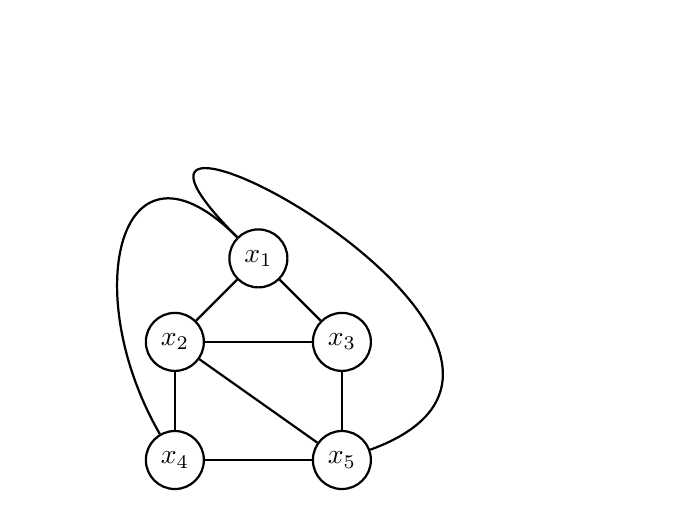
\begin{tikzpicture}[node distance={15mm}, thick, main/.style = {draw, circle}] 
            \node[main] (1) {$x_1$}; 
            \node[main] (2) [below left of=1] {$x_2$};
            \node[main] (3) [below right of=1] {$x_3$}; 
            \node[main] (4) [below of=2] {$x_4$}; 
            \node[main] (5) [below of=3] {$x_5$};
            \draw (1) -- (2);
            \draw (1) -- (3);
            \draw (2) -- (3);
            \draw (2) -- (4);
            \draw (3) -- (5);
            \draw (4) -- (5);
            \draw (2) -- (5);
            \draw (1) to [out=135,in=120,looseness=2] (4); % TODO: beautify
            \draw (1) to [out=135,in=20,looseness=3] (5); % TODO: beautify
        \end{tikzpicture} 
    \end{center}
\end{example}
